%
% File acl2018.tex
%
%% Based on the style files for ACL-2017, with some changes, which were, in turn,
%% Based on the style files for ACL-2015, with some improvements
%%  taken from the NAACL-2016 style
%% Based on the style files for ACL-2014, which were, in turn,
%% based on ACL-2013, ACL-2012, ACL-2011, ACL-2010, ACL-IJCNLP-2009,
%% EACL-2009, IJCNLP-2008...
%% Based on the style files for EACL 2006 by 
%%e.agirre@ehu.es or Sergi.Balari@uab.es
%% and that of ACL 08 by Joakim Nivre and Noah Smith

\documentclass[11pt]{article}
\usepackage[hyperref]{acl2018}
\usepackage{times}
\usepackage{latexsym}
\usepackage{url}
\usepackage{graphicx}
%\usepackage[
%	citestyle   = authoryear,           % use author-year citation
%	maxbibnames = 5,                    % maximum number of names printed in bibliography before truncation with ``et al.''
%	minbibnames = 1,                    % number of authors displayed if truncation happens
%	maxnames    = 4,                    % maximum number of names printed in citation before et al. is used
%	minnames    = 1,                    % number of authors displayed if truncation happens
%	datezeros   = false,                % no leading 0 if dates are printed
%	date        = long,
%	natbib      = true,                 % enable natbib compatibility
%	backend     = bibtex                % use bibtex as backend
%	]{biblatex}

%\addglobalbib{bibliography} % defines the name of the .bib file

\aclfinalcopy % Uncomment this line for the final submission
%\def\aclpaperid{***} %  Enter the acl Paper ID here

%\setlength\titlebox{5cm}
% You can expand the titlebox if you need extra space
% to show all the authors. Please do not make the titlebox
% smaller than 5cm (the original size); we will check this
% in the camera-ready version and ask you to change it back.

\newcommand\BibTeX{B{\sc ib}\TeX}

\title{LING 580/EE 596 Project \textemdash\ Malamute}
\author{Peter Schoener, Mingyi Yang, Xingyun Gao}

\date{}

\begin{document}
\maketitle
\begin{abstract}
	For our chatbot project, we designed an infobot for UW.
\end{abstract}

\section{Introduction}

\begin{quote}
	user: Who are you? \\
	malamute: I'm Malamute, an unofficial robo-dog tour guide!
\end{quote}

\subsection{Motivation}

The University of Washington, especially its Seattle campus, sees many visitors for a variety of reasons. As an educational institution, prospective students and their parents need to do due diligence before deciding on it. Current students may or may not know about what the city and the university have to offer, or may simply be interested in learning a bit of trivia. In addition, with its central location, architecture, and famous cherry trees, it is a tourist attraction.

While there are UW student ambassadors who present the university to these people, they are themselves students. As such, they only have a short time in which to get to know the university before they leave, meaning that they will necessarily not have as much information available as a computer could. Also, they will primarily know about the things that are relevant to current and maybe prospective students, but not necessarily parents or tourists. Although not relevant to tourists or current students, these student ambassadors will primarily be available in person.

All of these shortcomings could be addressed by an infobot. Moreover, part of the point of a student ambassador is to be the face of the intitution to the world. A good infobot, as a unique showcase of UW's already highly regarded computer science and computational linguistics programs, would be well-suited to just that. Therefore, we decided to attempt to build one for our project.

\subsection{Target Users}

As touched on above, there is a wide variety of target users. Prospective students need to learn about UW to be able to evaluate whether not only the academics but also the living situation and day-to-day circumstances align with their preferences. Their parents need to know the same, as well as, in many cases, what value they will be getting for their money. Equally, current students may not know about everything the university or its surroundings, and should in order to make the most of their time here.

Tourists, while the odd group out in terms of the sort of information they need, are also important to consider. They visit UW in substantial numbers, and will generally be interested in things like history, architecture, and scenery, with which the student ambassadors will have had less personal contact and, therefore, likely less expertise.

\section{System Architecture}

\begin{figure*}
	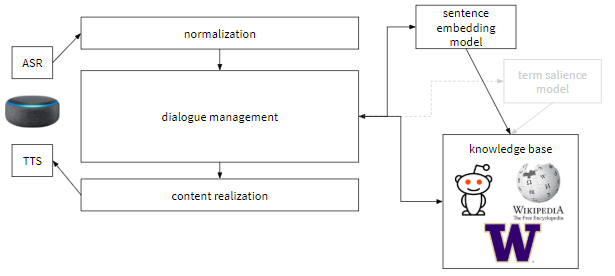
\includegraphics[width=\textwidth]{architecture.png}
	\caption{System architecture}
	\label{fig:architecture}
\end{figure*}

As shown in Fig. \ref{fig:architecture}, our system has more or less the standard layers of a chatbot. In the front end there are the ASR and TTS modules, handled by the Echo. In the backend, we have an embedding model and two knowledge bases drawn from internet data. Linking them we have normalization, dialogue management, and content realization modules.

\subsection{Middle End}

The middle end is quite simplistic, more or less directly linking the frontend and backend. Because this is a quickly implemented info bot, the dialogue control consists only of reprompts and a bit of initiative on the bot's part. After each answer, the bot will select from a few possible reprompts.

When the bot is unsure about the last answer, it will ask the user whether they would like to hear a bit of trivia and then select randomly from the primary knowledge base, again augmenting it with the secondary.

Before the query is passed in, however, it is normalized. We find that lowercasing alone drastically improves performance, and then removing numbers does not cause harm, but since the sentence vectorization does not discount punctuation we leave that in. For the surface realization, we experimented with the type of postprocessing used for the CLASSY \cite{classy} summarization model, but that turned out to be undesirable in a chatbot since it makes the sentences overly terse and, in the case of an infobot, sometimes strips away important information such as numbers.

In order to make the bot sound more human, the queries are fuzzed slightly after being vectorized, leading, in the case of multiple viable responses, to slight randomization. This is done simply by adding or subtracting a small amount to each dimension, in our case tuned to a maximum of $\frac{1}{38000}$. Over a 4800 dimensions, this leads to a non-negligible amount of noise.

\subsection{Backend}

Our backend is primarily a sentence embedding model. Specifically, it is a Python 3 reimplementation of the skipthoughts model \cite{kiros2015}. The vectors of the knowledge base are precomputed to save time and saved alongside it. The first knowledge database contains question-answer pairs. The user's query is checked against the questions in this knowledge base and the answer to the most similar question is selected. This is then combined with the most similar sentence to that answer from the larger knowledge base.

We had also added a module to fall back on in case there was no sufficiently similar question in the primary knowledge base. This was a tf-idf term salience model, which determines the most important words in the user's query and does a keyword search in the larger secondary database. It then selects the best sentence with one sentence of context before and after.

The second database is larger than the first, covering a larger variety of topics in more detail. However, it is completely unannotated, meaning that the information retrieval is much more difficult. Matching the user's query directly to a sentence in this database leads to terrible performance, and it turned out to even be difficult to find a cutoff at which the salience model was better than using just the first database.

\section{Data}

The data is drawn from Wikipedia, Reddit, and the UW website. The vectors are generated in advance for the sake of runtime efficiency and stored alongside the sentences. However, this does mean that they would need to be revectorized if new data were added.

The question and answer data in particular is drawn primarily from the UW website, with some samples from Reddit. This is because while the UW website has various FAQ pages, the Reddit forum format inherently lends itself to extracting question-answer pairs. As discussed in our paper presentation, it is relatively simple to extract this type of corpus from a forum, with viable techniques ranging from simply tagging all responses as answers to the original post question to those described in the presented paper \cite{huang}.

The primary corpus is also augmented with a few answers to conversational or ``joke'' questions. These include asking the bot which major it is in, how old it is, who it is, etc. These were added by hand, along with some rephrasings of poorly-worded questions.

We had initially experimented with an Alice/AIML-based bot, but this became difficult to extend according to our needs. We therefore dropped the Alice conversational elements, and the only smalltalk currently included in the bot is that which was added by hand to the primary dataset.

The secondary corpus is simply a list of sentences with parallel embeddings. These sentences are drawn from the UW website and Wikipedia. We had initially planned to crawl the entire UW website and certain Wikipedia pages (crawling techniques included following all links in the header section until a certain depth from the UW page), but this was then only done partly and by hand.

The primary dataset has just over a hundred question-answer pairs and is already quite good at answering most questions. It performed poorly in the demo because an old version of it was loaded instead of the then-current one. The secondary dataset contains about 42 kilobytes of sentences, for which the vectors, being 4800-dimensional floating point, take up several times more space.

\section{Evaluation}

We did not do any formal evaluation of this model, simply testing and progressively adjusting by ourselves. The weakness of this approach became immediately apparent during the demo; we had not prepared for all of the types of questions that were asked.

During the demo, more day-to-day type questions came up, specifically a request for dining recommendations on campus. Ironically, this was one of the types of questions that we had initially specified as what a human guide might be good at answering, in contrast to the more history and policy-oriented questions on which we focussed, as it turns out, too narrowly.

\section{Discussion}

\subsection{Strengths}

\begin{quote}
	user: What is the most popular major at UW? \\
	malamute: The most popular majors at University of Washington include: Social Sciences; Biological and Biomedical Sciences; Business, Management, Marketing, and Related Support Services; Engineering; and Health Professions and Related Programs. Is there any other information you would like to know? \\
	user: What does electrical and computer engineering study? \\
	malamute: Electrical and computer engineering is concerned with \ldots
\end{quote}

Even with a relatively small primary database, the bot is often able to find a good answer to an on-topic question. This was not entirely the case during the demo, with the wrong model being loaded and some of the questions being aimed at an overlooked domain (day-to-day living on campus, specifically food). However, the model is generally good at this.

Because of the nature of the dataset, with the responses being drawn more or less directly from the databases, the bot's outputs are always comprehensible and often even perfectly well-formed. This would not necessarily have been the case if we had opted for a more abstractive or understanding-based approach.

Our project is also easily extensible, both in terms of the code and the data. The code is largely modular, meaning that changing the parts related to the fallback mechanism, the dialogue management, etc. is quite simple. The data can be easily augmented with more sentences, especially the secondary database. The primary one would require more scraping, but even this could be made quite efficient with a good Reddit crawler.

The slight randomness introduced in the bot's responses was difficult to tune on vectors that large, but did turn out rather well. It changes its answers with noticeable frequency but not quite so wildly as to give wrong ones when the right one would be available.

Once started, the bot runs quite fast, responding almost instantly to a query. This is in large part due to the vectorization having been separated out; on a dataset this large it becomes slow enough to impede a conversation if it is redone each time.

\subsection{Weaknesses}

\begin{quote}
	user: How large is UW? \\
	malamute: UW is 157 years old. Amazing, isn't it? Do you want to know more about UW? \\
	user: I don't. \\
	malamute: You should come to UW! it's a great school. What else do you want to know?
\end{quote}

Due to the way that sentences are chosen, they sometimes interacy clunkily with those around them. For example, they may restate context present in the user's question, and indeed this is quite common; the overlap is part of what allows the sentences to be retrieved, but is then not stripped away in postprocessing. Also, the answers from the primary database do not always mesh seamlessly with the sentences from the secondary database.

The secondary database requires good and relevant embeddings in order to function. Because it was created by scraping and hardly sanitizing the webpages, it contains ``sentences'' which are actually just labels from UI elements or other site navigation features, which have embeddings that occupy the space outside of the relevant area. This means that queries that can not be matched to a UW-related sentence will simply be answered with nonsense.

Unfortunately, the bot does not handle smalltalk very well. Its ability to joke around with the user is limited to the few sentences in the primary database, and this combined with its very simple dialogue management make it quite robotic to interact with.

The more useful of the two databases, the annotated one, is very limited in size. It does not yet have the answers to all questions in all subdomains of UW, as we saw during the demo, and filling in this information will be somewhat tedious, although likely not difficult.

Once running the bot is quite quick to respond to a query, but the startup procedure involves loading the embedding model that will be used to get sentence embeddings for the queries, and that takes a non-negligible amount of time.

However, the main weakness of the model was its information retrieval system. The task of unsupervised retrieval turned out to be more difficult than we anticipated, and the bot struggles to find relevant answers to a question in the larger database.

\subsection{Future Work}

Most pressing of the future work, then is probably finding and implementing a more sophisticated information retrieval system. In parallel, both databases, first the annotated one and then the unannotated one, could stand to be rouded out. These two improvements, especially the former when combined with some tuning, would likely result in a massive boost in terms of performance.

The bot also needs more disfluencies and conversational cue support, if not a new dialogue management system. As it stands, it is a bit like a search engine with voice interactions, and so barely qualifies as a \textit{chat} bot.

Of course, the rest of the weaknesses mentioned above could also be addressed, but those should probably be given lower priority than the performance improvements.

\section{Team Member Contributions}

\subsection{Peter}

Peter suggested and implemented the embedding-based system. He also did some data collection and vectorized the data.

\subsection{Xingyun}

Xingyun wrote considerable parts of the final dialogue management system and had the idea for the tf-idf fallback module.

\subsection{Mingyi}

Mingyi was almost completely in charge of data collection. She also did substantial testing and troubleshooting.

% include your own bib file like this:
\bibliography{bibliography}
%\bibliographystyle{acl}
%\bibliography{bibliography}
\bibliographystyle{acl_natbib}

\end{document}
